\chapter{METODOLOGIAS E FERRAMENTAS}
\label{cap:elementos}

Para o desenvolvimento dos projetos foram utilizadas metodologias ágeis de desenvolvimento e ferramentas para desenvolvimento web (\textit{backend} e \textit{frontend}). Para entender melhor essas tecnologias as seções seguintes abordam cada uma delas.
\section{Metodologias Ágeis}

O "Manifesto ágil" surgiu em 2001 quando 17 conhecedores de metodologias ágeis se reuniram e discutiram como deveria ser o processo de desenvolvimento de software com metodologias ágeis, elencando 12 princípios que priorizam principalmente a satisfação do cliente, o trabalho em equipe, entregas de software mais rápidas e colaboração com o cliente. - \cite{manifestoAgil}

As metodologias ágeis são estratégias e comportamentos que devem ser seguidos afim de obter um resultado otimizado e mensurável. 
As principais metodologias ou \textit{frameworks} ágeis existentes são: 
Scaled Agile \textit{Framework} (SAFe) \cite{hayes2016scaling};
Feature Driven-Development (FDD)\cite{fdd};
Test Driven Development (TDD)\cite{beck2003test};
eXtreme Programming (XP) \cite{wildt2015extreme};
Dynamic Systems Development Method (DSDM) \cite{stapleton1997dsdm};
\textit{Kanban} \cite{boeg2010kanban};
entre outros.

No contexto do estágio descrito, \textit{Scrum} e \textit{Kanban} foram utilizadas e são descritas nas seções a seguir.
\subsection{\textit{Scrum}}

\textit{Scrum} é uma metodologia ágil que visa ter escopo fechado (número de tarefas predefinidas), calculadas através de métricas da equipe, como pontos de esforço.

Foi desenvolvida baseada nas metodologias de empresas do japão, como Toyota e Honda. É um \textit{framework} de trabalho que pode ser adaptado para diversas áreas.

As tarefas a serem desenvolvidas ficam armazenadas no \textit{product backlog}\footnote{Lista priorizada contendo as tarefas com uma breve descrição.}, sendo retiradas as com maior prioridade para serem inseridas na \textit{Sprint}.

Também existem alguns ritos que devem ser seguidos para o bom funcionamento do \textit{Scrum}, como as \textit{Daily Meetings, Planning, Review Meeting e Retrospective}, que ocorrem em um fluxo como ilustrado na Figura \ref{fig:scrum}.

\begin{figure}[H]
\centering
\caption{Fluxo \textit{Scrum}} %legenda
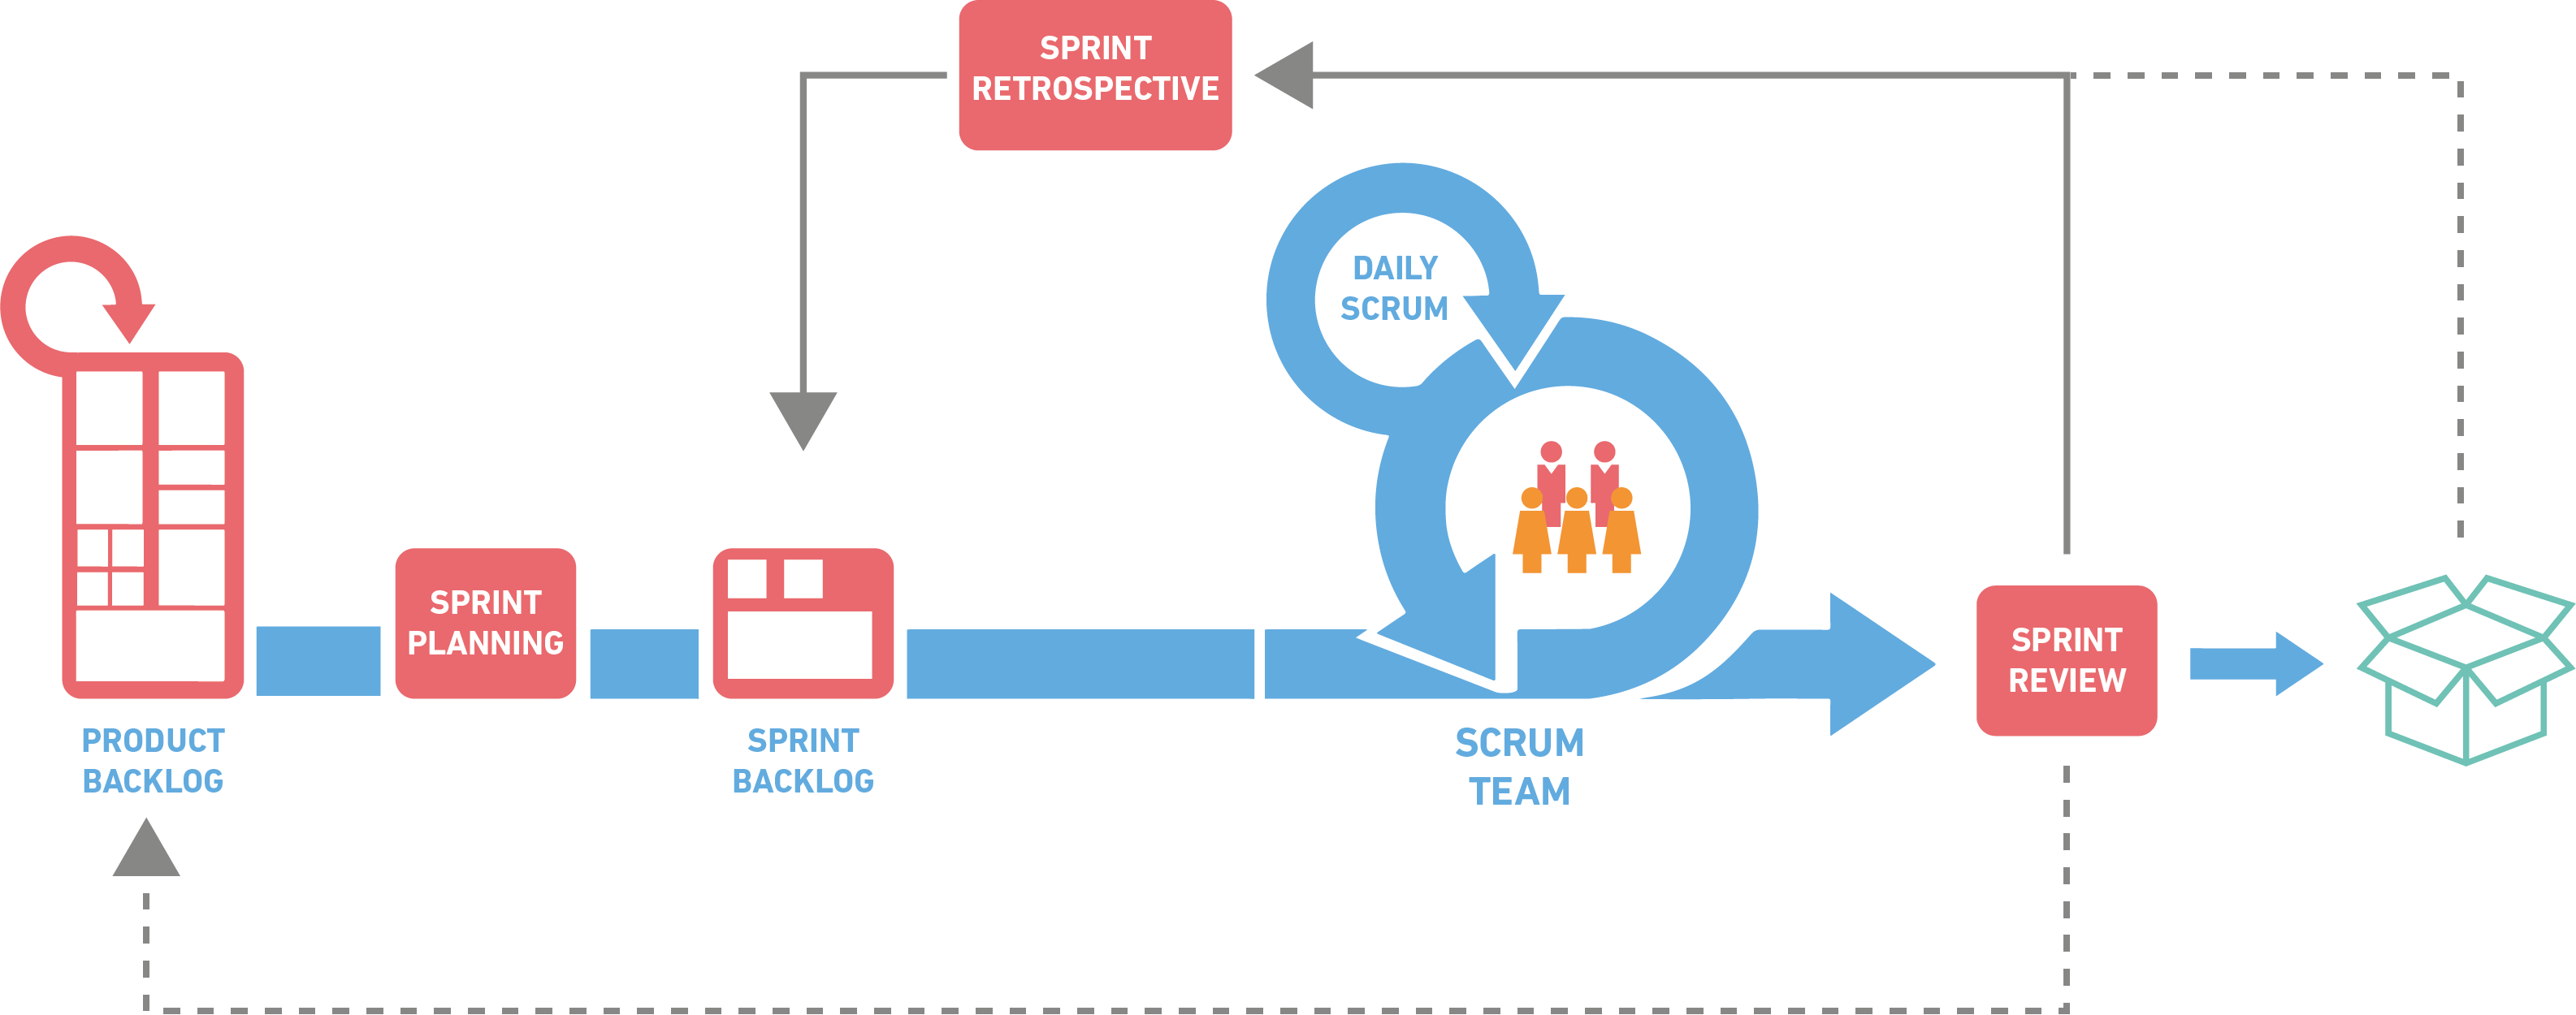
\includegraphics[scale=0.15]{Scrum}\\  % o 0.9 indica 90% do tamanho original
% pdfLaTeX aceita figuras no formato PNG, JPG ou PDF
% figuras vetoriais podem ser exportadas para eps e depois convertidas para pdf usando epstopdf
{\small Fonte:https://blog.mjv.com.br/frameworks-ágeis-saiba-como-funcionam-na-prática} %Fonte da imagem
\label{fig:scrum} %rotulo para refencia
\end{figure}

\textit{Daily Meetings} são reuniões diárias, rápidas e práticas para atualização da equipe sobre no que cada um está trabalhando, para um melhor entendimento da equipe.

\textit{Review Meetings} são reuniões feitas após o fim de cada \textit{Sprint}, para entender os resultados da equipe durante a \textit{Sprint}.

\textit{Retrospective} é uma reunião que ocorre todo fim de \textit{Sprint} para identificar o que funcionou e o que pode ser melhorado na \textit{Sprint}.

\textit{Planning} é a reunião que deve ser feita antes de cada \textit{Sprint} para definir quais atividades devem ser desenvolvidas, entender melhor sobre elas, descrevendo-as minuciosamente e prevendo possíveis problemas.
Quem gerencia esse \textit{product backlog} é o  ~\nameref{sec:po}, que cuida de organizar, definir e priorizar as tarefas.

Muitas vezes separadas em \textit{Sprints} (tempo pré-definido pela equipe, geralmente de 10 dias úteis), as tarefas são incluídas em um quadro e devem ser finalizadas no prazo previsto.

\begin{quote}
  \textit{Scrum} é um \textit{framework} simples e pequeno e, assim, funciona bem em  cada contexto se for utilizado em conjunto com outras técnicas e praticas a serem experimentadas e adaptadas. - \cite{sabbagh2014scrum}
\end{quote}
\begin{quote}
  O \textit{Sprint} é o ciclo de desenvolvimento, onde o incremento do produto pronto é gerado pelo Time de Desenvolvimento a partir dos itens mais importantes do Product Backlog. - \cite{sabbagh2014scrum}
\end{quote}


\subsubsection{\textit{Scrum Master}}

Cargo que tem como função cuidar das obrigações impostas sobre a metodologia \textit{Scrum}, como lembrar dos ritos, marcar reuniões e garantir o bom desenvolvimento das atividades estabelecidas para a \textit{Sprint}.

\begin{quote}
Garante que o time esteja
totalmente funcional e
produtivo.

Facilita a colaboração entre as
funções e áreas e elimina os
impedimentos do time.

Protege o time de
interferências externas.

Garante que o processo está
sendo seguindo. Participando
das reuniões diárias, revisão
da \textit{Sprint}, e planejamento. \cite{sabbagh2014scrum}

\end{quote}

\subsubsection{Analista de Qualidade(Tester)}

Responsável por encontrar problemas e possíveis melhorias durante o desenvolvimento, garantido o funcionamento total do sistema para que seja validado com o cliente.

\subsubsection{Gerente de projetos(GP)}

Cargo que tem como função gerenciar os projetos e times da sua
 tribo\footnote{Conjunto de desenvolvedores e outros cargos que cuidam de um ou vários projetos.}, cuidando para que sejam entregues os requisitos no prazo combinado.

\begin{quote}
  O gerente de projetos é a pessoa destacada e designada como principal responsável por atingir os objetivos do projeto. - \cite{cruz2013scrum}
\end{quote}
\subsubsection{\textit{Product Owner(PO)}}
\label{sec:po}
Cargo que tem como função cuidar do relacionamento do time com o produto,
 definindo e priorizando requisitos.
 
 \begin{quote}
  Define os requisitos do
  produto, decide a data de
  release e o que deve conter
  nela.

  É responsável pelo retorno
  financeiro (ROI) do produto.
  
  Prioriza os requisitos de
  acordo com o meu valor de
  mercado.
  
  Pode mudar os requisitos e
  prioridades a cada \textit{Sprint}.

  o Aceita ou rejeita o resultado de
  cada \textit{Sprint}. - \cite{sabbagh2014scrum}
 \end{quote}

\subsection{\textit{Kanban}}
\textit{Kanban} é uma opção de metodologia ágil mais adaptativa, tendo escopo aberto torna-se possível inserir atividades durante o tempo.
Muitas vezes é comparado a uma tubulação de água, onde existe uma determinada quantidade de água a ser transportada, porém é necessário definir o tamanho do tubo ou vazão, sendo essa a quantidade, a quantidade de esforço que a equipe consegue trabalhar.
Assim como o \textit{Scrum}, possui um backlog controlado por um Product Owner. As atividades são inseridas assim que libera a vazão, como em uma tubulação.
Diferentemente do \textit{Scrum}, não há necessidade de \textit{Reviews} e \textit{Retrospective} uma vez que não possui \textit{Sprints}, porém algumas reuniões para analisar o desempenho da equipe são um boa prática.
Geralmente é determinado um máximo de esforço e, ao final de uma atividade, é inserida uma nova com prioridade.

O \textit{Kanban}, como ilustra a Figura \ref{fig:kanban}, é um quadro onde as tarefas são organizadas em filas de acordo com seu estágio de execução: Novo, Pronto, Em Andamento, Pronto para testar, Em teste, Terminado.
Cada  tarefa é definida com um identificador, descrição da atividade, pessoa responsável e prioridade. As tarefas podem ser movimentadas de uma fila para outra de acordo com seu estado de execução.

\begin{figure}[H]
\centering
\caption{Quadro \textit{Kanban}} %legenda
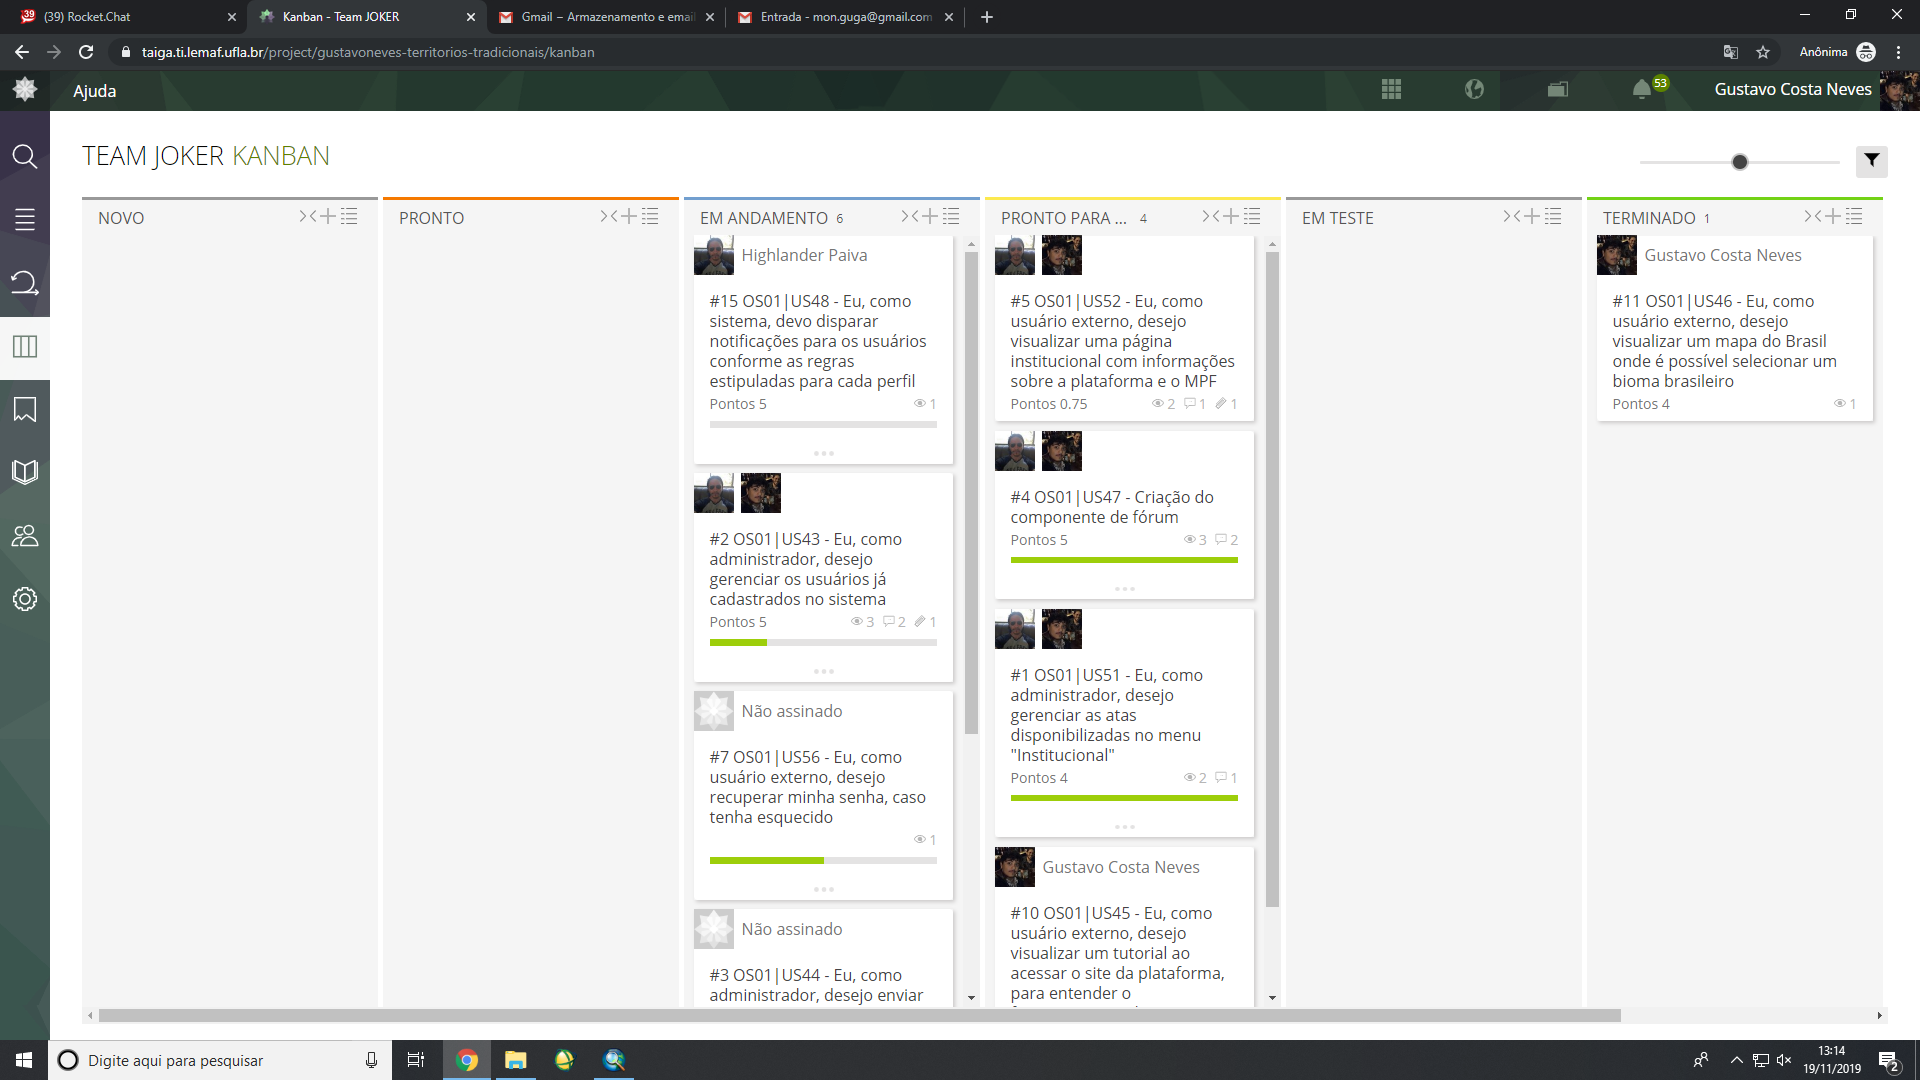
\includegraphics[scale=0.2]{quadroKanban}\\  % o 0.9 indica 90% do tamanho original
% pdfLaTeX aceita figuras no formato PNG, JPG ou PDF
% figuras vetoriais podem ser exportadas para eps e depois convertidas para pdf usando epstopdf
{\small Fonte: https://taiga.ti.LEMAF.ufla.br/} %Fonte da imagem
\label{fig:kanban} %rotulo para refencia
\end{figure}

\section{\textit{Frameworks}}

Para facilitar o desenvolvimento, diversas ferramentas foram criadas e durante o desenvolvimento de novos projetos foi necessária a utilização das mesmas.

As aplicações que utilizam esses \textit{frameworks} geralmente são separadas em \textit{frontend} e \textit{backend} devido à arquitetura cliente-servidor que é utilizada para o desenvolvimento das aplicações. O cliente é o agente responsável por enviar mensagens requisitando algum serviço ao serviço e é conhecido como front-end, pois é a parte que interage diretamente com o usuário. 

O servidor é o agente responsável por realizar as operações necessárias para
responder as requisições do lado cliente da aplicação, sendo também conhecido
como \textit{backend}.
Essa definição facilita o desenvolvimento modularizado da aplicação, uma vez que o \textit{backend} pode ser utilizado por diversos \textit{frontend}. Isto facilita a modularização das aplicações, uma vez que um \textit{backend} pode ser utilizado por diversos \textit{frontend}.

\subsection{Frontend}

Nessa seção são apresentados frameworks para front-end utilizados pelo LEMAF.

\subsubsection{AngularJS}

AngularJS é um \textit{framework} open-source, de desenvolvimento front-end, que possibilita o desenvolvimento de aplicações web.

Teve sua primeira versão lançada em 2010 pela Google.

\begin{quote}
  o AngularJS foi criado por Miško Hevery e Adam Abron  em  2009  e  é  um  \textit{framework}  JavaScript open  source(código  aberto), client-side(do lado  do  cliente)  que  promove  uma  alta  produtividade  na  experiência  do  desenvolvimento Web - \cite{ferreira2018analise}
\end{quote}


\subsubsection{VueJS}

VueJS é um \textit{framework} JavaScript de open-source, focado no desenvolvimento de interfaces de usuário e aplicativos de página única.

Teve sua primeira versão lançada em 2014.

\begin{quote}
  Vue é uma lib/\textit{framework} JavaScript reativo, para  o  desenvolvimento  de  componentes  que,  por  sua  vez,  são  códigos  que  podem  ser reaproveitados em sua aplicação - \cite{ferreira2018analise}
\end{quote}


\subsubsection{ReactJS}

O React é uma biblioteca JavaScript, open-source, com foco em criar interfaces de usuário em páginas web. É mantido por empresas como Facebook e Instagram e uma comunidade de desenvolvedores individuais. 

Teve sua primeira versão lançada em 2013.

\begin{quote}
  Segundo a sua documentação(2018), ele é, na  verdade,  uma  biblioteca  de  UI  (User  Interface),  representando  apenas  a  camada view do Model  View  Controler(MVC).  - \cite{ferreira2018analise}
\end{quote}

\subsection{Backend}

É a parte da aplicação que é inacessível ao usuário, onde é controlado todo o sistema (autenticação, regras de negocio, jobs e etc).

\subsubsection{\textit{Play Framework}}

O Play \textit{Framework} é uma alternativa "limpa" de esticar as stacks do Java Enterprise. Ele se concentra na produtividade do desenvolvedor e tem como objetivo arquiteturas RESTful. 

O objetivo da estrutura do Play é facilitar o desenvolvimento de aplicativos da web, mantendo o Java.

Teve sua primeira versão lançada em 2009.

\begin{quote}
\textit{Play! Framework} 2 é planejado para ser "full stack" e completamente integrada, a boa notícia é que não há requisitos específicos para você ou meu ambiente começar a criar novos aplicativos da web. - \cite{petrella2013learning}
\end{quote}

\subsubsection{\textit{Spring Boot}}

O Spring é um \textit{framework} open-source para a plataforma Java criado por Rod Johnson e descrito em seu livro "Expert One-on-One: JEE Design e Development".
Trata-se de um \textit{framework} baseado nos padrões de projeto inversão de controle e injeção de dependência.

Teve sua primeira versão em 2002.

\begin{quote}
  Spring \textit{Framework} é um \textit{framework} voltado para desenvolvimento de aplicações corporativas para a plataforma Java, baseado nos conceitos de inversão de controle e injeção de dependências. - \cite{weissmann2014vire}
\end{quote}

\subsubsection{\textit{DotNet Framework}}

O \textit{.NET Framework} é uma iniciativa da empresa Microsoft, que visa uma plataforma única para desenvolvimento e execução de sistemas e aplicações.
Todo e qualquer código gerado para .NET pode ser executado em qualquer dispositivo que possua um \textit{framework} de tal plataforma.

Teve sua primeira versão lançada em 2002.

\begin{quote}
  
O .Net \textit{Framework} é um \textit{framework} de desenvolvimento que fornece uma nova interface de programação para serviços e APIs do Windows e integra várias tecnologias que surgiram da Microsoft no final dos anos 90. \cite{thai2003net}
\end{quote}

\subsection{Banco de Dados}

É aonde ficam armazenadas informações necessárias para o funcionamento das aplicações.

\subsubsection{Postgresql}

É um sistema gerenciador de banco de dados desenvolvido na linguagem de programação C.
Gerencia banco de dados relacionais e possui ótimo desempenho.

Possui extensões que contribuem com sua eficacia, como por exemplo o POSTGIS, uma extensão que possibilita o Postgresql a utilizar dados Geoespaciais.
Um das vantagens é que sua licença é gratuita desde fins estudantis a empresariais.
Teve sua primeira versão lançada em 2009.

\begin{quote}
  O PostgreSQL é uma das opções de banco de dados, pois se trata de um servidor SGBD de grande potencial e confiabilidade, contendo todas as características dos principais bancos de dados utilizados no mercado. Uma das suas características são suas licenças para uso gratuito, seja para fins estudantis seja para a realização de negócios, possibilitando que empresas o utilizem livremente. \cite{postgres}
\end{quote}

\section{TECNOLOGIAS}
\label{cap:conclusao}

Durante o estágio, tive a possibilidade de testar e utilizar diversas tecnologias e \textit{frameworks}, com foco especial em tecnologias \textit{frontend}.
Para melhor entendimento do trabalho, é necessário um dissertação sobre as mesmas.

Os \textit{Frameworks} principais de \textit{frontend} são ReactJS, Angular e Vuejs.
Sendo ReactJS e VueJS os principais em favoritos dentro da comunidade do GitHub\footnote{Comunidade de desenvolvedores onde se é possível compartilhar e discutir sobre projetos e tecnologias.} como demonstrado na figura \ref{fig:github}

\begin{figure}[H]
\centering
\caption{Comparação frameworks front-end pelo github} %legenda
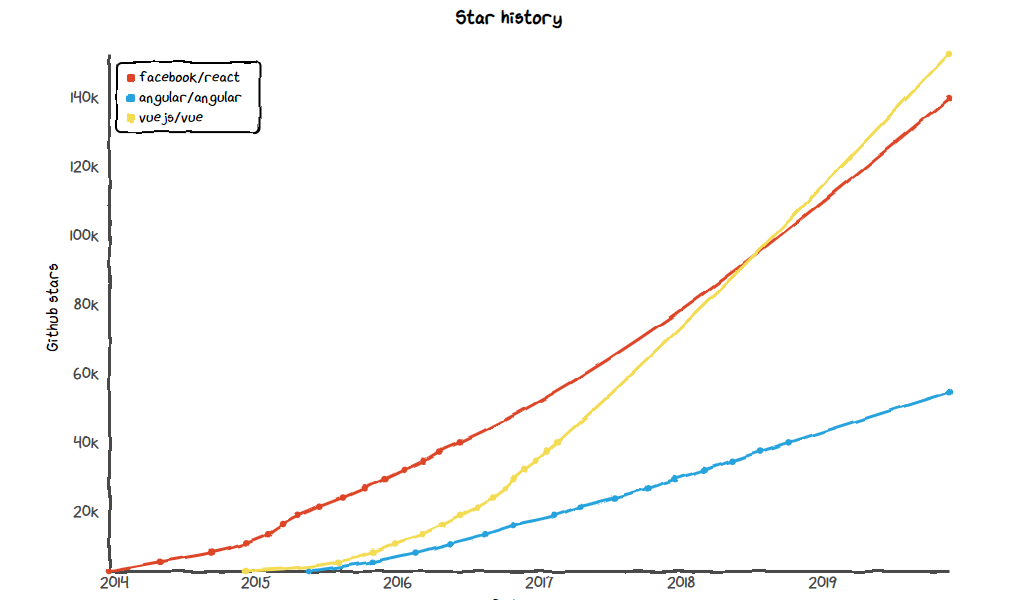
\includegraphics[scale=0.55]{githubFramework}\\  % o 0.9 indica 90% do tamanho original
\label{fig:github} %rotulo para refencia
{\small Fonte: https://star-history.t9t.io} %Fonte da imagem
\end{figure}

Com seu lançamento tardio em relação ao ReactJS, o VueJS vem crescendo e neste ano de 2019 ultrapassou o numero de estrelas no github, enquanto o \textit{framework} Angular
 cresce de forma lenta e continua.

Os \textit{frameworks} VueJS e ReactJS tinham como grande diferencial o uso da Virtual DOM\footnote{É um framework para manipulação do DOM} em vez da DOM(\textit{Document Object Model})\footnote{é a representação dos compomentes na página}. Uma vez que a DOM era uma abstração do codigo HTML, a DOM Virtual é uma abstração da DOM.

Enquanto a DOM é uma árvore de objetos interligados, com diversas conexões e ramificações, onde modificações simples nas mesmas eram muito frequentes. Já a DOM virtual veio para 
solucionar este problema, ela já possui configurações e implementações do \textit{browser}, livrando o desenvolvedor de ter que configurá-las manualmente. Além disto a DOM virtual é mais leve e simples, sendo mais fácil compreende-la e desenvolve-la.

Outro grande diferencial graças a esta mudança, é que a abstração de componentes se tornou mais inteligente, uma vez que era possível desenvolver componentes desacoplados e acoplados somente onde eram necessários.

No início do estágio, diversos projetos que tive contato eram utilizado Angular, por conta de ter sido lançado em 2010 pela Google. Foi uma grande evolução, uma vez que projetos mais velhos foram desenvolvidos em Flex, que era uma tecnologia para interfaces em flash com integração com Java.

O \textit{framework} Angular facilitava absurdamente o trabalho como desenvolvedor, uma vez que em diversos casos, que seriam necessárias diversas linhas de Jquery e Javascript, era somente necessário o uso de uso de uma, como exemplificam os códigos da Figura \ref{fig:exemplocodigo1} e a Figura \ref{fig:exemplocodigo2} que adicionam um evento a elementos DOM pelo JQuery e VirtualDOM pelo Angular.


\begin{figure}[!htb]
\centering
\caption{Adicionando evento a elementos DOM pelo JQuery} %legenda
\begin{lstlisting}
var box = $( "#box" );
$( "#botao" ).on( "click", function( event ) {
    box.show();
});
\end{lstlisting} 
\label{fig:exemplocodigo1} %rotulo para refencia
\end{figure}

\begin{figure}[!htb]
\centering
\caption{Adicionando evento a elementos VirtualDOM pelo Angular} %legenda
\begin{lstlisting}
<div ng-show={show} ng-click={() => {show = true}}/>
\end{lstlisting} 
\label{fig:exemplocodigo2} %rotulo para refencia
\end{figure}
    

Como a base de desenvolvedores no LEMAF já possuia muita experiência com Angular, foi difícil fazer com que adotassem outras tecnologias em outros projetos.

Porém logo após iniciativa e insistência de um desenvolvedor, apresentamos o VueJS para a organização do LEMAF e conseguimos com que os projetos fossem desenvolvidos com ele.

O VueJS não possuia documentação vasta como o do Angular, porém possuia atualizações recorrentes, porém com sua acensão, foi fácil demonstrar que em alguns anos a documentação dele seria melhor que a do Angular.

Porém era complicado mesmo assim, pois a credibilidade de um \textit{framework} da Google contra a de um ex-desenvolvedor da Google(Criador do VueJS) era incomparável, era realmente um risco a mudança. 
Mas ao mostrar que o projeto recebia uma grande verba de patrocínio, a curva de crescimento e que o mesmo possuia uma equipe fixa de pelo menos 50 contribuidores, entenderam que o risco não era tão grande.

A adesão ao VueJS foi muito bem aceita em diversas equipes, pois a flexibilidade que ele proporciona ao desenvolvedor comparado ao Angular era gigantesca, com a possibilidade de configuração quase infinita, diversas bibliotecas e varios modos de arquitetura, o VueJS se tornou foco de estudo na empresa.
Uma das iniciativas vindas dos organizadores da empresa foi fornecer alguns cursos da plataforma Alura para desenvolvimento web com VueJS.

Sua performance mesmo com sendo maior que o ReactJS demonstrava mais fluidez, desde a ferramenta de \textit{hot-reload}\footnote{Recarregamento quente, possibilita que a DOM seja recarregada somente nos locais de modificação, sem ser necessário o recarregamento da tela total.}, até a compilação para modo produção.
Sua arquitetura era simples e direta, centralizada em poucos arquivos e ao mesmo tempo separava bem os comportamentos. Sua documentação era bem escrita, descrevendo os ciclos de vida dos componentes até suas diretivas.

Muitos aprenderam por conta própria facilmente, uma vez que a complexidade abaixava, tendo toda a estrutura de um componente do Angular com 5 arquivos, em 1 arquivo .vue somente.
Como vários módulos do LEMAF já utilizavam de Pug/Jade em vez do HTML puro, a transição foi muito tranquila, pois VueJS já suportava Pug e diversas outras linguagens.

Outro grande benefício encontrado durante a transição foram as bibliotecas de UI\footnote{User Interface Design - é uma área de design que planeja e analisa os modos de iteração do usuario com o sistema.}, pois com Angular o mais adequado era o uso do Material Design que já era da própria empresa ou 
Bootstrap\footnote{Framework para desenvolvimento de componentes e front-end para sites e aplicações web usando HTML, CSS e JavaScript.}, porém com o VueJS vieram varias outras bibliotecas como Vuetify e ElementUI, que tornaram as interfaces bem mais leves, modernas e bonitas, saindo daquele estilo antigo e estático.

Também foi apresentado pela equipe de design, eu e outro desenvolvedor, a ideia de Design System para a organização, que era algo que seria fácil de ser aplicado graças ao VueJS, que tinha um otimo suporte a componentização e que se usado 
de forma correta(Separando componentes de visualização e logica), poderia melhorar significantemente o tempo para desenvolvimento dos projetos.

Em 2019, vendo o advento das tecnologias de desenvolvimento hibrido para mobile, foi questionado a equipe se seria interessante o uso de \textit{frameworks} mais próximos, para possíveis futuros projetos.
Dai a adesão ao ReactJS, já que o principal utilizado para desenvolvimento mobile era o ReactJS-native, que se assemelhava bastante.

Ao estudarmos sobre, entendemos que a curva de aprendizado para quem desenvolvia VueJS iria ser bem pequena, já que ambos eram bem flexíveis.

Ele era mais leve que o VueJS que já era muito leve e ainda possuia uma documentação muito boa.
porém um grande diferencial que existia era o uso do JSX, uma versão do Javascript que combina elementos do HTML dentro do Javascript. Era bem legível e bem similar ao HTML, mas não tinha um bom suporte para Pug.

Mesmo com este problema, resolvemos testar um projeto pequeno com ele. 

As primeiras semanas foram difíceis, tivemos que estudar muito sobre o \textit{framework} pois ele possuia diversas bibliotecas que melhoravam significantemente meu uso.

Após as duas primeiras semanas o desenvolvimento fluiu, as duvidas eram pouco recorrentes e as respostas eram fáceis de encontrar. porém voltamos ao problema inicial do Angular, 
a falta de um biblioteca de UI que combinasse com a identidade da empresa.

Foi colocado então em prática a construção do Design System, um processo de construção de identidade visual para empresa, com componentes próprios desenvolvidos com excelência para poderem ser utilizados em varios projetos, facilitando o desenvolvimento de todos e garantindo qualidade.

A criação dessa biblioteca tinha como objetivo fazer com que os desenvolvedores centralizassem os componentes, contribuindo publicamente com a biblioteca, sendo mais fácil corrigir um erro e depois atualizar a biblioteca que resolve-lo em todos projetos.

E isto tornou-se prazeroso com ReactJS, pois o suporte para componentização por ele é ótimo, desde o desenvolvimento até a criação dos testes automatizados.
